\documentclass[a4paper]{article}

\usepackage{INTERSPEECH2016}

\usepackage{graphicx}
\usepackage{amssymb,amsmath,bm}
\usepackage{textcomp}
\usepackage{booktabs}

\def\vec#1{\ensuremath{\bm{{#1}}}}
\def\mat#1{\vec{#1}}


\sloppy % better line breaks
\ninept

\title{TTIC 31220 Final Project: \\ Toward a Reduced-Form Factor Portfolio}

%%%%%%%%%%%%%%%%%%%%%%%%%%%%%%%%%%%%%%%%%%%%%%%%%%%%%%%%%%%%%%%%%%%%%%%%%%
%% If multiple authors, uncomment and edit the lines shown below.       %%
%% Note that each line must be emphasized {\em } by itself.             %%
%% (by Stephen Martucci, author of spconf.sty).                         %%
%%%%%%%%%%%%%%%%%%%%%%%%%%%%%%%%%%%%%%%%%%%%%%%%%%%%%%%%%%%%%%%%%%%%%%%%%%
%\makeatletter
%\def\name#1{\gdef\@name{#1\\}}
%\makeatother
%\name{{\em Firstname1 Lastname1, Firstname2 Lastname2, Firstname3 Lastname3,}\\
%      {\em Firstname4 Lastname4, Firstname5 Lastname5, Firstname6 Lastname6,
%      Firstname7 Lastname7}}
%%%%%%%%%%%%%%% End of required multiple authors changes %%%%%%%%%%%%%%%%%

\makeatletter
\def\name#1{\gdef\@name{#1\\}}
\makeatother \name{{\em Kabir Sawhney, Joseph Denby}}
\address {\small \tt \{ksawhney, jgdenby\}@uchicago.edu}

%\twoauthors{Karen Sp\"{a}rck Jones.}{Department of Speech and Hearing \\
%  Brittania University, Ambridge, Voiceland \\
%  {\small \tt Karen@sh.brittania.edu} }
%  {Rose Tyler}{Department of Linguistics \\
%  University of Speechcity, Speechland \\
%  {\small \tt RTyler@ling.speech.edu} }

%
\begin{document}

  \maketitle
  %

  \section{Introduction}

    The returns on different financial assets are influenced by a similar set of underlying risks. These risks include macroeconomic variables, such as inflation and GDP growth, and market factors, including company size and relative value. In financial theory, the return of any given asset can be modeled as a linear combination of returns on these risks, with different weights on different risks for each asset, plus an error term. However, there is no consensus set of risk factors, and a great deal of research has gone into studying what the appropriate set of risk factors are from which asset returns are constructed.
    \par Some researchers have applied linear dimensionality reduction techniques to large factor universes, with a focus on linear PCA, to statistically derive latent factor representations. The goal of our project is to extend this work using non-linear dimensionality reduction, with a focus on the techniques learned in the course. 
    \par To study this question, we found a set of factors designed to replicate returns to macroeconomic and financial market risks over time. We applied dimensionality reduction to this data, then used the lower-dimensional representation as an input to a linear regression model with stock returns as the response variable. We found that, when seeking to predict returns on the broad equity market and individual stocks, non-linear dimensionality reduction generally did not perform better than linear PCA or our theoretically-constructed benchmark.

  
  \section{Related Work}

   The inspiration for our project came from Kozak, Nagel, and Santosh (2017) [1], who argued that reduced-form factor models tend to perform well empirically in predicting asset prices. In their paper, the authors use linear PCA to derive a low-dimensional factor representation, from a set of factors defined by Novy-Marx and Velikov (2015) [2]. Then, they show that the principal components derived from their analysis perform about as well as their benchmark, the Fama-French three-factor model [3], in explaining the variation in returns on the portfolios they examined.
   \par We used the data from Novy-Marx and Velikov [2] as the basis for our analysis. Their set of 24 factors focuses on market-based risks, defining strategies to capture the returns to factors including company size, relative value, momentum, and profitability; full definitions for each factor are provided in the referenced paper. These factors were dynamic, with the portfolios of assets designed to replicate the returns regularly adjusted as asset weights naturally rise and fall with prices. A dynamic, rules-based strategy construction method should provide a closer approximation to the actual return of each factor over time, as asset weights are adjusted as they become more or less correlated with the relevant factor. However, the drawback of this strategy is that it leaves our analysis vulnerable to flaws in Novy-Marx and Velikov's methodology. 
   \par Other authors have applied PCA to a variety of different types of financial data. A\"{i}t-Sahalia and Xiu (2015) [4] apply PCA to high-frequency data, analyzing the covariance structure of the constituents of the S\&P 100 Index on a microsecond-by-microsecond level. Kim and Jeong (2005) [5] analyzed a correlation matrix of stocks that traded on the New York Stock Exchange, and attempted to derive qualitative explanations for what the first few principal components meant. They asserted that the first principal component represented a market-wide influence which affected all stocks, the next few represented effects on different groups of stocks, and the remaining ones indicated randomness in price fluctuations.
   \par In our review, we found linear PCA being applied to a very wide range of different data sets and research problems, but did not find any analysis which sought to apply any other dimensionality reduction technique. The explanation for this gap seems to be the difficulty of interpretation when using non-linear techniques -- principal components derived using the eigenvector method generally have a theoretical analogue, while components derived using other methods don't necessary lend themselves easily to interpretation.
   
   \section{Methods}
   \par Our basic methodology was to apply various representation learning techniques to a set of portfolio risk factor dimensions, use the low dimensional representations to train linear regression models predicting the returns of various stocks, and compare the techniques using the $R^2$ value of each resulting regression model. We use $R^2$ as our metric as it is easily interpretable as a means of comparison between linear regression models and is a standard metric in the relevant literature (e.g., [1]). 
   \par Our target data consisted of monthly stock returns for Procter \& Gamble, United Technologies, Exxon-Mobil, 3M, and IBM, in addition to monthly returns for the S\&P 500 index, all between July 1963 and December 2013. We sourced the data from Wharton Research Data Services [6]. We opted for a collection of individual stocks instead of solely the index because the Fama-French model includes overall market returns as a factor, making it unsuitable for comparison with other methods. We also believed that we might find some interesting results using individual stocks; the literature generally focuses on portfolio returns, but a method for predicting specific stock returns would be of interest to financial market participants. We picked these companies for their size and longstanding history on the stock market; they have enough returns data to allow for robust analysis using our representation methods.
   \par An initial consideration in our analysis concerned the potential presence of autocorrelation in either of our datasets. This is often an issue in financial analysis, particularly when dealing with data at fine levels of temporal granularity (e.g., daily, hourly returns). However, brief analysis on our datasets revealed that autocorrelation was largely a non-issue; lagged returns did not produce any significant gains when included as predictors in our regression models. 
   \par Our set of representation learning techniques incorporated a broad range of nonlinear methods: Kernel PCA with RBF and polynomial kernel functions, Isomap, and spectral embedding using Laplacian eigenmaps. By means of comparison, we also used a standard linear PCA model. Additionally, we trained linear regression models using the three-factor Fama-French dataset to get a sense of how our learned representations perform relative to a widely-used benchmark.
   \par To train and evaluate our representation learning models, we split our dataset into training, development, and test sets (50\%/25\%/25\%). Our split was done in time to simulate how this analysis would apply to real-world prediction settings;  predicting future returns can only incorporate past data. Specifically, for most models our hyperparameter tuning pipeline was as follows: the training dataset was used to train the representation learning model, then the tuning dataset was transformed to a lower dimensional representation and used to fit a linear regression model with the accompanying output data. For spectral embedding, since this method cannot train on one dataset and transform another, we combined the training and development sets to fit the model and transform the data into a reduced representation; this reduced form was then fed into a regression model like other representation learning methods.
   \par We tuned hyperparameters for each method by varying the value and plotting the resulting linear regression model's $R^2$ value for each stock's development set. For most hyperparameters, we decided on values by picking whatever configuration resulted in the largest $R^2$ result (i.e., which representation produced the best linear regression model.) However, when picking the number of components, we aimed for a middle value that produced good results while still reducing dimensionality by a non-trivial amount. Our decisions for these hyperparmeters were done qualitatively by observing resulting $R^2$ plots; we looked for a 'knee' in the collective stock trajectories suggesting diminishing returns in performance with increased components.
   
   \begin{figure}[t]
   	\centering
   	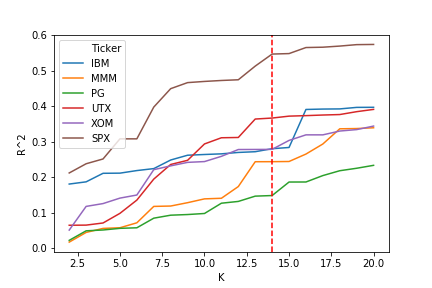
\includegraphics[width=\linewidth]{linPCA_tune.png}
   	\caption{{\it Tuning Components for Linear PCA.}}
   	\label{fig:LinPCATuning}
   \end{figure}
   
   \begin{figure}[t]
   	\centering
   	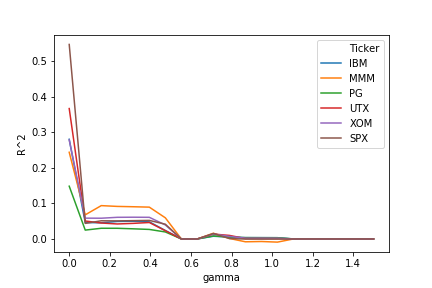
\includegraphics[width=\linewidth]{rbf_gamma_tune.png}
   	\caption{{\it Tuning Gamma for RBF KPCA.}}
   	\label{fig:RBFGammaTuning}
   \end{figure}
   
   \begin{figure}[t]
   	\centering
   	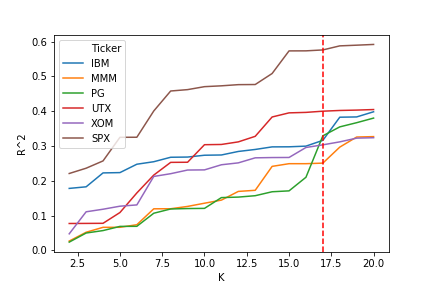
\includegraphics[width=\linewidth]{KPCA_tune.png}
   	\caption{{\it Tuning Components for RBF KPCA.}}
   	\label{fig:RBFComponentTuning}
   \end{figure}
   
    \begin{figure}[t]
    	\centering
    	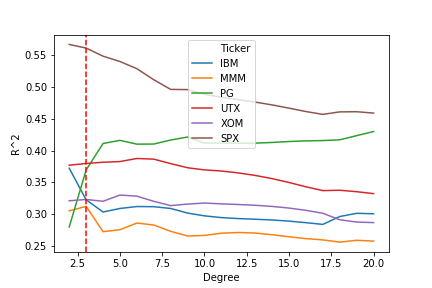
\includegraphics[width=\linewidth]{poly_degree_tune.png}
    	\caption{{\it Tuning Degree for polynomial KPCA.}}
    	\label{fig:PolyDegreeTuning}
    \end{figure}
   
   \begin{figure}[t]
   	\centering
   	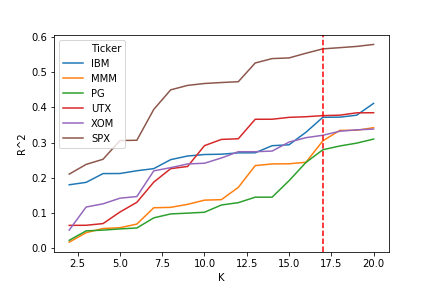
\includegraphics[width=\linewidth]{poly_components_tune.png}
   	\caption{{\it Tuning Components for polynomial KPCA.}}
   	\label{fig:PolyComponentTuning}
   \end{figure}
   
   \section{Results}
   \par Our linear PCA representation appeared to yield optimal performance with 14 components (Figure \ref{fig:LinPCATuning}), producing $R^2$ between $.1$ and $.35$ for each individual stock.  
   \par Kernel PCA with the RBF kernel performed best with $\gamma \approx 0$ (Figure \ref{fig:RBFGammaTuning}), with $R^2$ falling precipitously with increased regularization. Following this, the RBF Kernel representation with 17 components appeared to yield optimal performance (Fibure \ref{fig:RBFComponentTuning}), producing $R^2$ between $.2$ and $.55$.
   \par Kernel PCA with the RBF and polynomial kernels performed approximately the same. The polynomial kernel yielded optimal performance with a 3rd degree polynomial (Figure \ref{fig:PolyDegreeTuning}), but performance was nearly identical to the RBF Kernel with varying component values (Figure \ref{fig:PolyComponentTuning}.)
   \par Our Isomap implementation used a K nearest neighbors graph construction; tuning yielded consensus optimal performance with $K= 24$ (Figure \ref{fig:IsomapKNNTuning}). Our Isomap representation performance appeared to level with 12 components (Figure \ref{fig:IsomapComponentTuning}), producing $R^2$ values between $.1$ and $.35$.
   \par Our spectral embedding method performed eigendecompositon on a graph Laplacian matrix constructed via K nearest neighbors. Tuning the number of nearest neighbors (for graph construction) yielded a consensus optimum at $K=70$ (Figure \ref{fig:SpectralKNNTuning}.) With this implementation, performance appeared to reach a consensus optimum with 12 components (Figure \ref{fig:SpectralComponentTuning}.)
   \par Figure \ref{fig:TestResults} plots the $R^2$ values for linear regression models trained using the optimal configurating of each representation learning method predicting each ticker. From this, we see that the two Kernel PCA methods yield optimal performance for every stock, but only marginally better than linear PCA on whole. Isomap yields worse performance on every stock except 3M, and spectral embedding yields by far the worst performance of any representation learning method. Finally, the Fama-French five-factor model outperforms all low-dimensional representations for 3M and United Technologies, approximately matches performance for Exxon-Mobil, and underperforms most methods for IBM and Procter \& Gamble. See Table \ref{tab:results} for complete results.
    \begin{figure}[t]
    	\centering
    	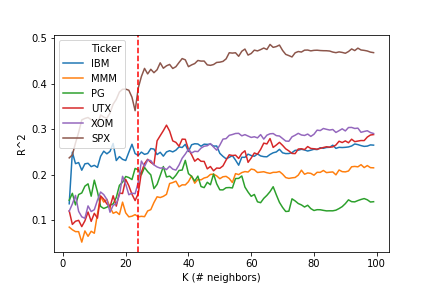
\includegraphics[width=\linewidth]{isomap_knn_tune.png}
    	\caption{{\it Tuning Nearest Neighbors for Isomap.}}
    	\label{fig:IsomapKNNTuning}
    \end{figure}
    
    \begin{figure}[t]
    	\centering
    	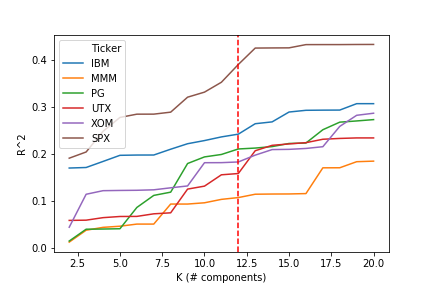
\includegraphics[width=\linewidth]{isomap_tune.png}
    	\caption{{\it Tuning Components for Isomap.}}
    	\label{fig:IsomapComponentTuning}
    \end{figure}
    
    \begin{figure}[t]
    	\centering
    	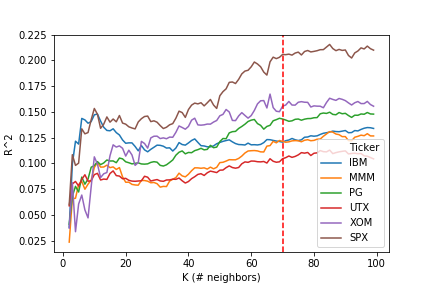
\includegraphics[width=\linewidth]{spectral_knn_tune.png}
    	\caption{{\it Tuning Nearest Neighbors for Spectral Embedding.}}
    	\label{fig:SpectralKNNTuning}
    \end{figure}
    
    \begin{figure}[t]
    	\centering
    	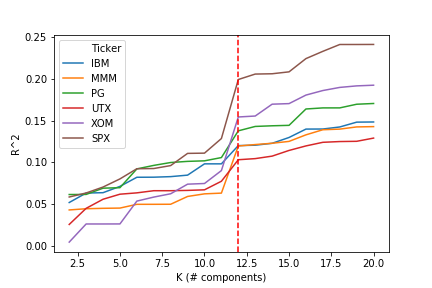
\includegraphics[width=\linewidth]{spectral_tune.png}
    	\caption{{\it Tuning Components for Spectral Embedding.}}
    	\label{fig:SpectralComponentTuning}
    \end{figure}
    
        \begin{table}
        	\caption{\label{tab:results} {\it $R^2$ results on test dataset. \textbf{Bold} indicates best result.}}
        	\vspace{2mm}
        	\centerline{
        		\resizebox{\columnwidth}{!}{
        			\begin{tabular}{lrrrrrr}
        				\toprule            Method &       IBM &       MMM &        PG &       UTX &       XOM &       SPX \\
        				\midrule               FF5 &  0.350 &  0.409 &  0.107 &  0.494 &  0.207 &  0.986 \\
        				LinearPCA &  0.451 &  0.182 &  0.234 &  0.383 &  0.210 &  0.570 \\
        				RBF\_KPCA &  \textbf{0.478} &  0.186 &  \textbf{0.234} &  \textbf{0.391} &  \textbf{0.236} &  \textbf{0.577} \\
        				Poly\_KPCA &  \textbf{0.478} &  0.186 & \textbf{ 0.234} &  \textbf{0.391} &  \textbf{0.236} &  \textbf{0.577} \\
        				Isomap &  0.406 &  \textbf{0.209} &  0.160 &  0.371 &  0.217 &  0.514 \\
        				SpectralEmbedding &  0.081 &  0.082 &  0.116 &  0.081 &  0.085 &  0.142 \\
        				\bottomrule
        			\end{tabular}
        		}}
        		
        	\end{table}
        	
        	
        	\begin{figure}[t]
        		\centering
        		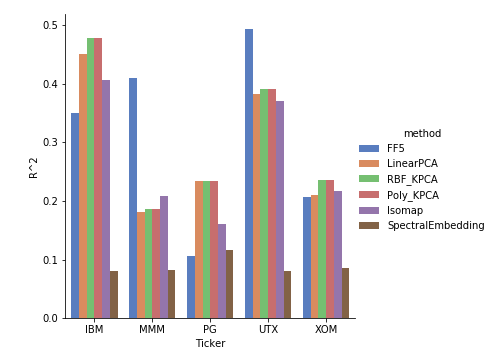
\includegraphics[width=\linewidth]{test_results.png}
        		\caption{{\it Test Results by Ticker and Method.}}
        		\label{fig:TestResults}
        	\end{figure}
    
    \section{Discussion}
    \par Our main finding was that, for deriving a low-dimensional factor model to predict monthly returns on individual stocks, non-linear dimensionality reduction approaches do not offer an advantage over linear PCA. For the six assets we tested, in only one case did a non-linear approach have a better $R^2$ on the test set than the linear approach, when the derived factors using Isomap performed slightly better than linear PCA on the return data for Procter \& Gamble. Among the non-linear techniques we tested, we got the best performance using kernel PCA with the radial basis function kernel, followed by Isomap. We also tested spectral embedding, but got very poor linear regression results with that method.
    \par A surprising finding was that improvement in $R^2$ on the validation set leveled off at a relatively high number of principal components. For all of our dimensionality reduction methods, we chose 12-17 components for our latent representation after tuning – however, most existing research in the field has found that the latent dimensionality for factor analysis should a relatively small number, and certainly less than 10. As described above, we chose to focus on individual stocks, while most existing research focuses on portfolios and market indices – because individual stocks are more variable, it requires more components to accurately predict returns. We saw this result in our analysis, as the number of principal components to get good performance on the S\&P 500 was lower than the number for individual stocks.
    \par Comparing our results to those using the Fama-French three-factor model, our results were mixed. For two of the stocks, Fama-French performed much better than empirical results derived using PCA; for two others, Fama-French performed much better; and for the last one, our PCA representations outperformed. However, given that our lower-dimensional representation had components in the teens compared to three for Fama-French, it is safe to conclude that their theoretically-derived model is better than our empirically-derived one, at least when using the Novy-Marx and Velikov data as the underlying set.
    \par The factor model approach does not seem to work well for predicting individual stock returns, at least when using monthly returns data. Both our models and the Fama-French three-factor model generally could not explain more than 40\% of the variation in the data, and often much less than that. As discussed in a previous section, we chose to focus on individual stock returns because we didn't find any existing work in applying these models to individual companies, and whether they could be applicable would be of interest to market participants. Based on these results, it makes sense for researchers to focus on broader indices and portfolios, as individual stocks appear to have too much variation to be well represented by any manageably sized model.
    \par The result of not getting an improvement in explanatory power using non-linear methods is evidence in favor of the idea that the fundamental relationship among different risk factors is linear. We would expect to see significant improvement in performance when using non-linear dimensionality reduction if our data lies in a non-linear subspace or manifold, and would expect the opposite if our data naturally lies close to a linear subspace. This result may be an explanation for why linear PCA is the overwhelming choice of technique for dimensionality reduction in the literature - it is possible that researchers have previously tried the non-linear approach but found that factor data can generally be well represented by a linear subspace.
    
    \section{Future Work}
    \par The most frequent piece of feedback we got on our results throughout the project concerned qualitative interpretations of our learned representations, both linear and non-linear. This question is definitely of interest, as it would be very useful to know which factors or groups of factors (whether market-driven, macroeconomic, etc.) had more influence on returns for different companies. However, we found that conducting this analysis might have taken more analytical effort than the project itself – even getting to a starting point would require a great deal of exploratory analysis on a variety of different potential underlying risk factors. We think this question could be an interesting extension of our work, especially in exploring whether there is the possibility of deriving an explanation for learned non-linear representations. One of the reasons why we believe non-linear techniques are underrepresented in the literature is precisely because it is very challenging to interpret learned non-linear representations.
    \par Another extension of our work could be to repeat the same analysis, but with a different set of underlying factors and/or with more frequent data. As mentioned in our introduction, different authors have proposed a wide range of different factor bases to predict financial asset returns, and we only analyzed one in this project. It also would have been interesting to see if we could have gotten different results if we had data on a more frequent time scale. Most of the papers we reviewed used daily or intraday price data, but we were not able to get access to this level of detail.
    
    \section{Acknowledgements}
    KS wrote the proposal and update. KS sourced the data. JGD and KS imported and cleaned the data. JGD built the representation learning and regression pipelines and produced plots and tables. JGD and KS performed tuning experiments, made final model selections, prepared the presentation, and wrote up the final report. Thanks to Bowen Shi and Karen Livescu for their input and guidance!   


  \newpage
  \eightpt
  \bibliographystyle{IEEEtran}

%\bibliography{mybib}

  \begin{thebibliography}{9}
    \bibitem[1]{Factor-Models}
      Serhiy Kozak, Stefan Nagel, and Shrihari Santosh,
      ``Interpreting Factor Models,''
      \textit{Journal of Finance}, vol.~73, no.~3, pp.~1183--1223, 2018.
    \bibitem[2]{Novy-Marx}
      Robert Novy-Marx and Mihail Velikov,
      ``A Taxonomy of Anomalies and Their Trading Costs,''
      \textit{The Review of Financial Studies}, vol.~29 no.~1, pp.~104--147, 2016.
    \bibitem[3]{FF}
      Eugene F.\ Fama and Kenneth R.\ French,
      ``Common risk factors in the returns on stocks and bonds,''
      \textit{Journal of Financial Economics}, vol.~33 no.~1, pp.~3--56, 1992.
    \bibitem[4]{AitSahalia}
    Yacine A{\"i}t-Sahalia and Dacheng Xiu,
    ``Principal Component Analysis of High Frequency Data,''
    \textit{National Bureau of Economic Research Working Paper Series}, Working Paper 21584, 2015.
    \bibitem[5]{Kim Jeong}
    Dong-Hee Kim and Hawoong Jeong,
    ``Systematic analysis of group identification in stock markets,''
    \textit{Physical Review E}, vol.~72: 046133, 2005.
     \bibitem[6]{WRDS}
	Wharton Research Data Services. ``CRSP Monthly Stock,'' wrds.wharton.upenn.edu, accessed 03/01/2019.
	\bibitem[7]{RNM Data}
	Robert Novy-Marx. ``Data used in A Taxonomy of Anomalies and Their Trading Costs,'' rnm.simon.rochester.edu/data\_lib/index .html, accessed 03/01/2019.
  \end{thebibliography}

\end{document}
